\section {Systematic Uncertainties on the Search}

The source of systematic uncertainties are considered as following:
\begin{itemize}
\item Jet Energy Scale (JES)
\item Jet Energy Resolution (JER) 
\item Choise of Background Parametrization
\item Luminosity
\end{itemize}
Our procedure to evaluate the first three of these is to use a smooth fit to the 
QCD background as a data sample, and to find the cross section upper limits for 
this data sample before and after systematic shifts as described below. 

\subsection{Jet Energy Scale (JES)} 
The uncertainty on the JES that is important for this analysis
is the uncertainty on how well the dijet resonance simulation models the jet energy scale of real jets.
If the simulation produces jets with too high a response, then the true position of the expected resonance
peak for that resonance mass would really be at lower mass than predicted by the simulation. The JES uncertainty
is only on the simulation of the resonance, as the background 
comes directly from the data via the fit and therefore has the same JES as the data.
For this preliminary prompt-reco dataset we use older and more conservative uncertainties on the 
jet energy scale~\cite{PAS_JME_10-010} essentially 5\% over our dijet mass region.
We expect these uncertainties to be significantly reduced to about 2-3\% uncertainty in dijet 
mass when we have the official jet energy calibration for 2011, since we were able to achieve that value at
the end of the 2010 run~\cite{PAS_JME_10-011}.
Conceptually, shifting the 
resonance lower in dijet mass by the jet energy scale uncertainty 
gives more background from QCD and therefore a larger upper limit on the resonance cross section.

%\begin{figure}[!ht]
%  \begin{center}
%   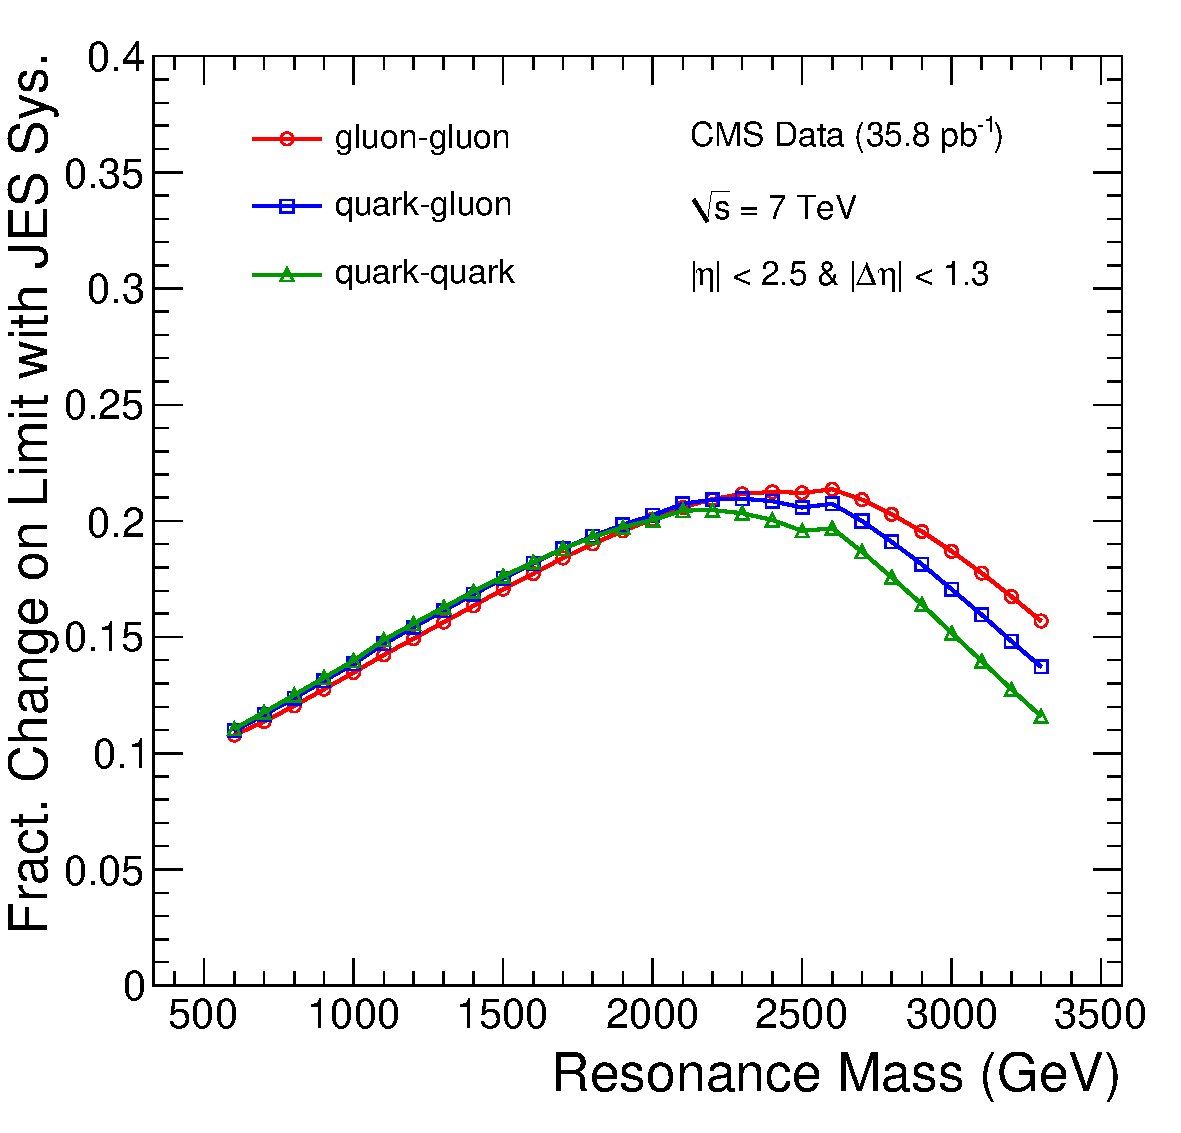
\includegraphics[width=\textwidth]{Figures/Fractional_Change_JES_All.pdf}
%    \caption{ 
%Fractional change in the expected uppper limit on the cross section for qq, qg
%and gg resonances from a JES systematic shift of 3-5\%.}
%    \label{JES}
%  \end{center}
%\end{figure}
%\clearpage

\subsection{Jet Energy Resolution (JER)}

The uncertainty on JER at high dijet mass is $\pm10\%$~\cite{JME-10-014-PAS}.  
The tails of the resolution function are in good agreement between data and MC.
This same dijet asymmetry method with a varying cut on the 3rd jet pt constrains the differences in 
radiation between the data and MC, and thereby constrains differences in MC 
modeling of the resonance shape due to radiation to be small.
We therefore take the uncertainty on JER to be roughly $\pm10\%$, and assume that the signal is being smeared 
by a Gaussian which increases the core resolution by 10\%. A comparison of resonance shapes are shown in
Fig.\ref{conv_shape}.

\begin{figure}[!ht]
  \begin{center}
         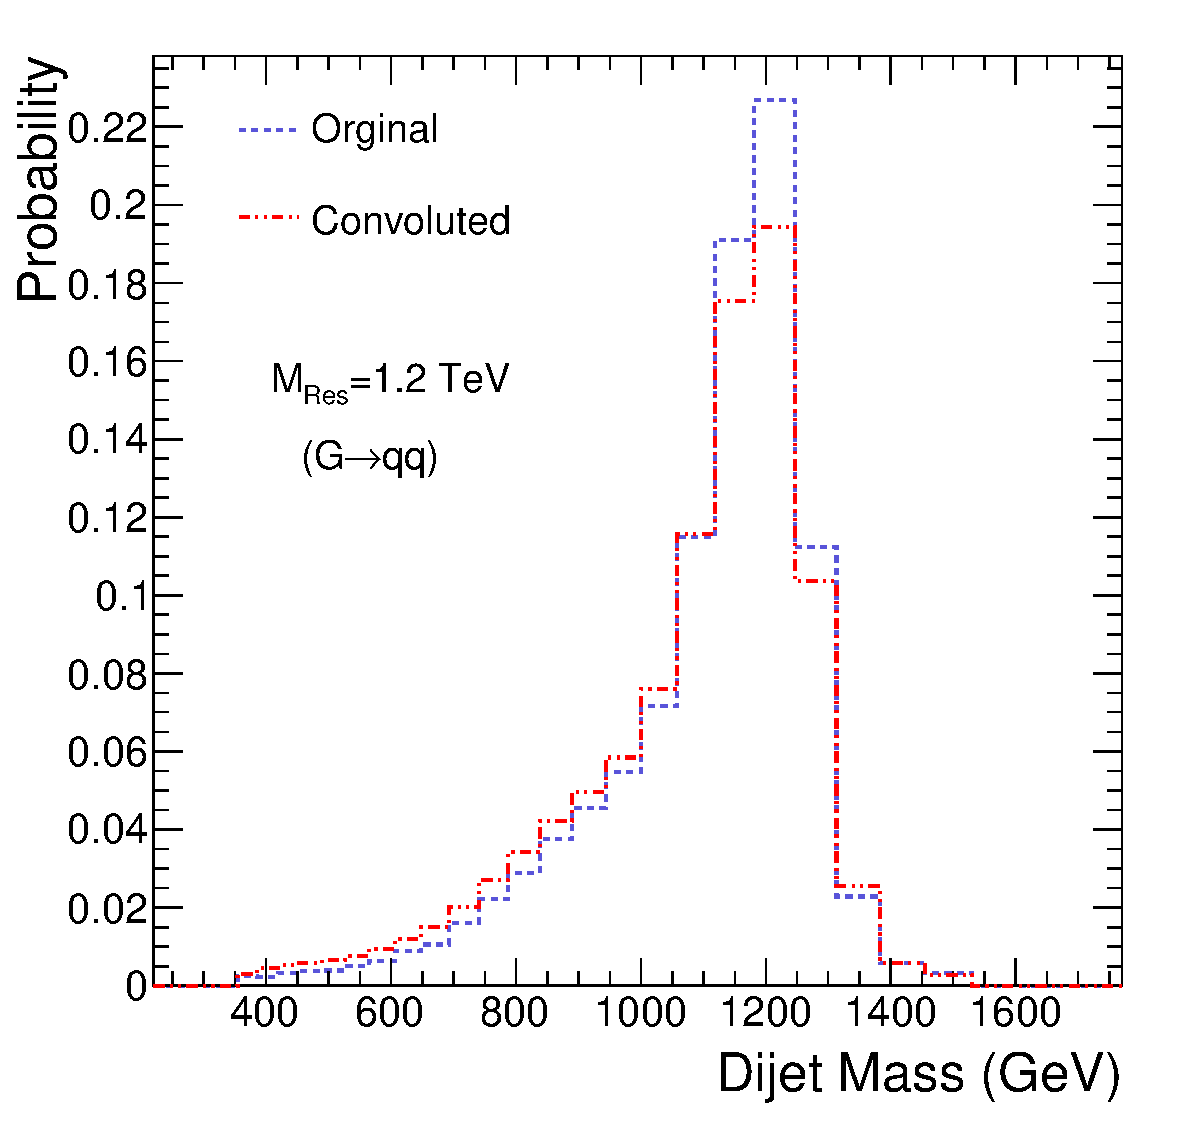
\includegraphics[width=0.3\textwidth]{Figures/Resonace_Shape_Convoluted_qq_1200_2.pdf}
          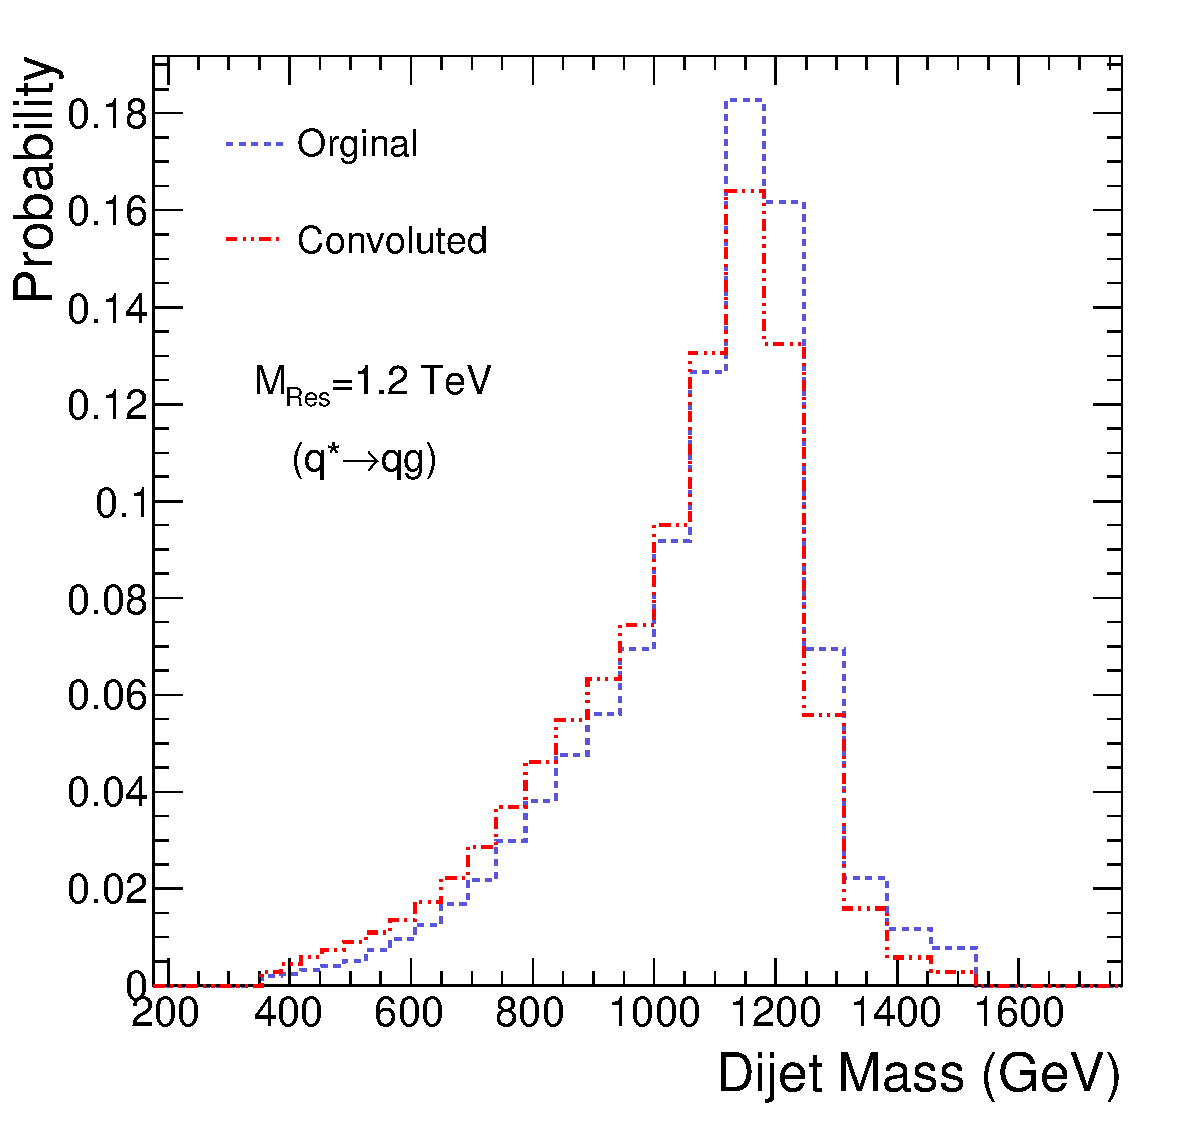
\includegraphics[width=0.3\textwidth]{Figures/Resonace_Shape_Convoluted_qg_1200_2.pdf}
           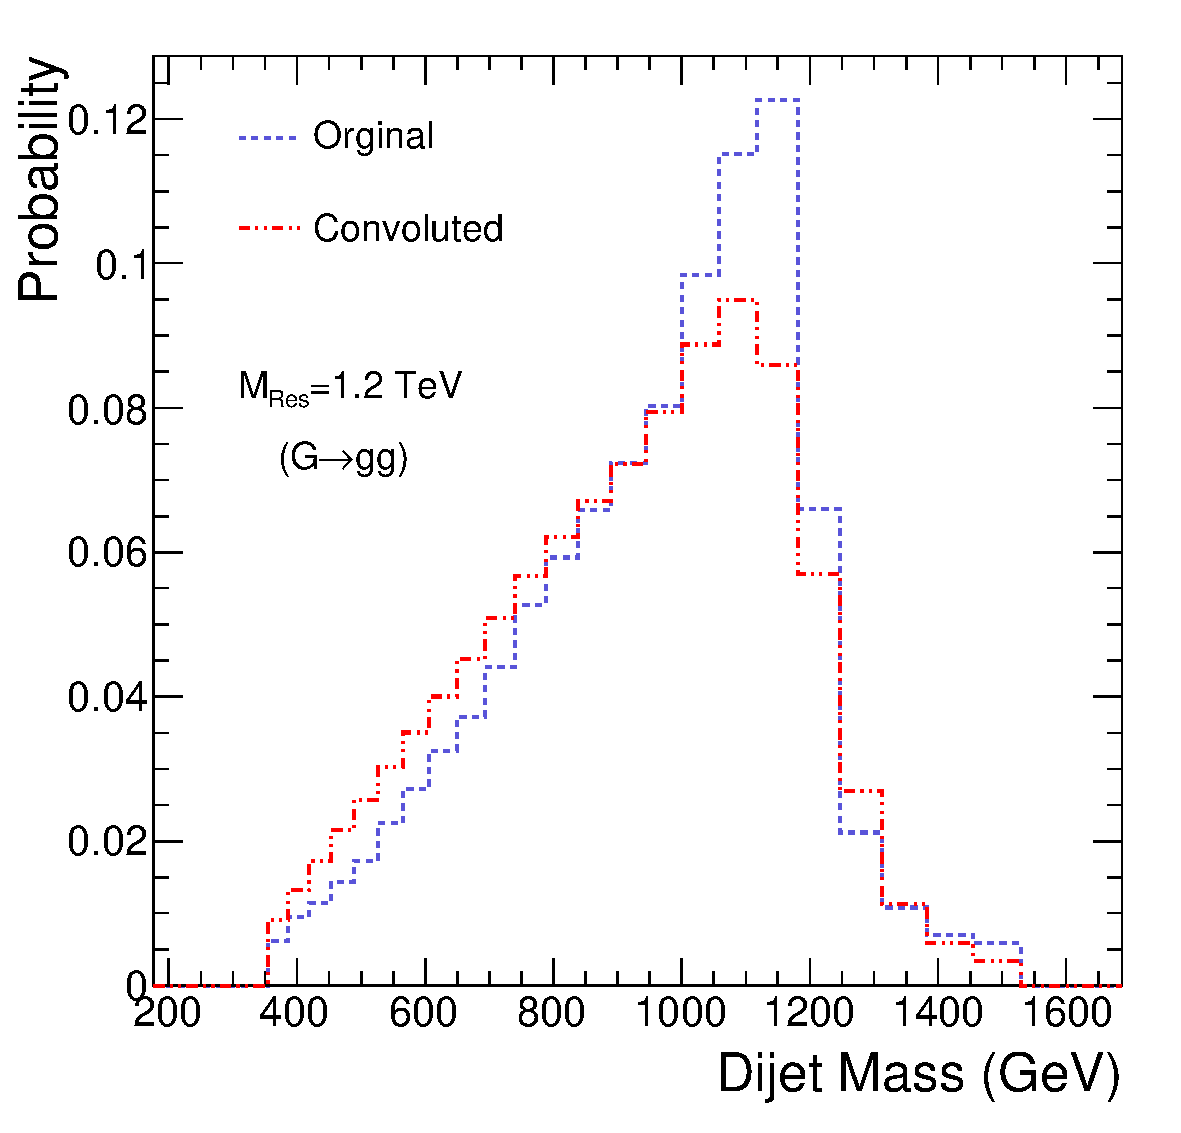
\includegraphics[width=0.3\textwidth]{Figures/Resonace_Shape_Convoluted_gg_1200_2.pdf}
    \caption{Resonance shape comparison before and after convolution for a $1.2$ TeV resonance 
    of type qq (left), qg(middle) and gg (right).}
    \label{conv_shape}
  \end{center}
\end{figure} 

Resolution of the Gausian core of the resonance signal as a function of resonance
mass was illustrated in Fig.~\ref{resolution}. The resolution is calculated as 
$\sigma/mean$, where $\sigma$ and the $mean$ are obtained from the Gaussian fit to the dijet mass distribution.

%\begin{figure}[!ht]
%  \begin{center}
%    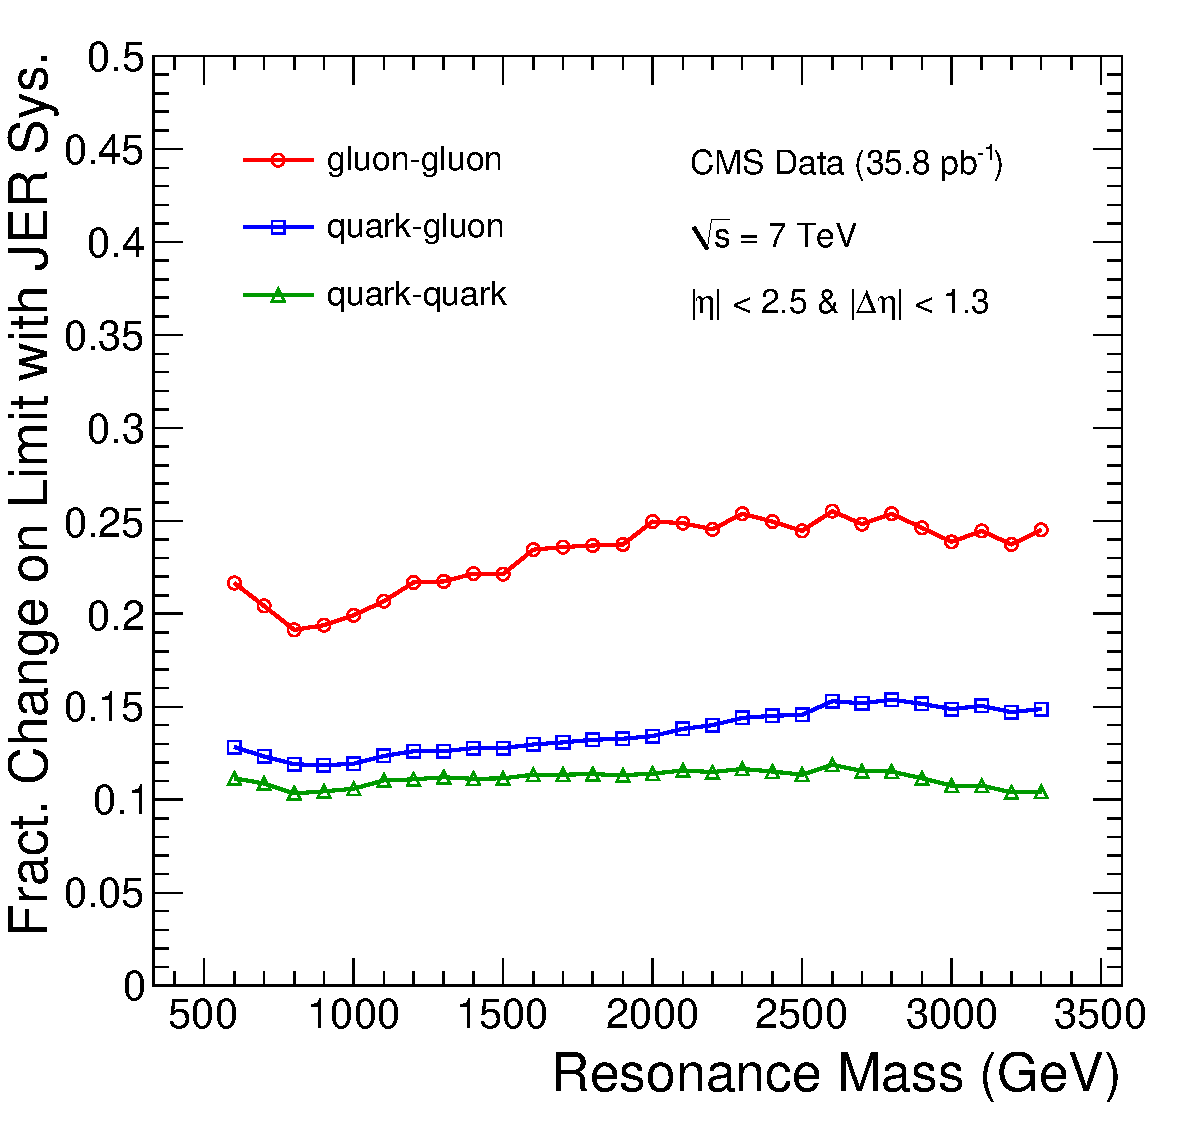
\includegraphics[width=\textwidth]{Figures/Fractional_Change_JER_All.pdf}
%    \caption{Fractional change on limit with JER systematic uncertainty.}
%    \label{JER}
%  \end{center}
%\end{figure}


\subsection{Background Parameterization}
For the background parameterization, we consider the change in the level of the
background when varying the fit parameters by $1\sigma$. We vary the three shape 
parameters in the fit simultaneously, taking into account their correlation. The
parameters were fully correlated, or fully anti-correlated, so we moved them all 
by $1\sigma$ simultaneously with the appropriate sign.

\subsection{Luminosity}
The uncertainty on the integrated luminosity is 4\%.


\subsection{Incorporating Systematics in the Limit}

The above mentioned systematic uncertainties are included
in the limit as nuisance parameters as discussed in the statistical model Appendix~\ref{appStatModel}
and implemented in Appendix~\ref{appStatImplement}.
To summarize briefly, we effectively integrate over these nuisance parameters, and the uniform prior, 
to find the 95\% CL upper limit including systematic uncertainties. 
Our 95\% CL upper limit both with statistical uncertainties only and including systematic 
uncertainties  for all three resonance types, and the fractional change in the limit with a breakdown of
the contributoin of each systematic for qg resonances only, 
are shown separately in Fig.~\ref{limit_change_calo}-\ref{limit_change_fat} for calo, pf and fat jets.

We note that in the 2010 paper systematics were included using an adhoc conservative method. For that paper 
smooth systematics as a function of resonance mass wer found for JES, JER and background from fits to smoothed
datasets with 1$\sigma$ shifts in the signal.  The total systematic in signal cross section was found by 
adding all in quadrature. Posterior distribution functions were convoluted with systematics and gave smooth
changes.  

We now use a fully Bayesian method as discussed in Appendix~\ref{appStatModel} and ~\ref{appStatImplement}.
This process uses the data more directly when incorporating the systematics.  The effect of the systematics
depends directly on the data, which is not smooth. Changes in the limits from systematics are not expected 
to smoothly vary with resonance mass using this procedure, and they do not.  Truly Bayesian systematics can
sometimes improve the limit slightly.

We note that the effect of systematics shown in Fig.~\ref{limit_change_calo}-\ref{limit_change_fat} is generally small.  
The dominant systematic is usually the JES
uncertainty, as expected.  At resonance masses that correpond to upward fluctuations of the data above the fit,
the JES systematic can actually improve the limit, as it effectively moves the resonance shape to dijet mass 
values where there is less indication of a signal in the data.  For some values of resonance mass the background
systematic is the dominant systematic, and can be a large effect, producing a sudden change in the limit at certain
values of resnance mass.  We have determined that this happens where the fit parameter uncertainty allows a lot
more signal to be pushed into the fit.  This often happens where the fit is poorly constrained by multiple points
in a row that lie right on top of the fit, fitting much better than they need to given their larger statistical 
errors. In those situations the shape can be dramatically altered without much statistical penalty, because the
fit is already too good where all the points line up right on top of the fit.  In these regions we sometimes get
a large background systematic.  


%We note that for both string resonances and excited quarks, the mass limits are reduced by only
%0.1 TeV by including systematics.

\begin{figure}[!ht]
  \begin{center}
     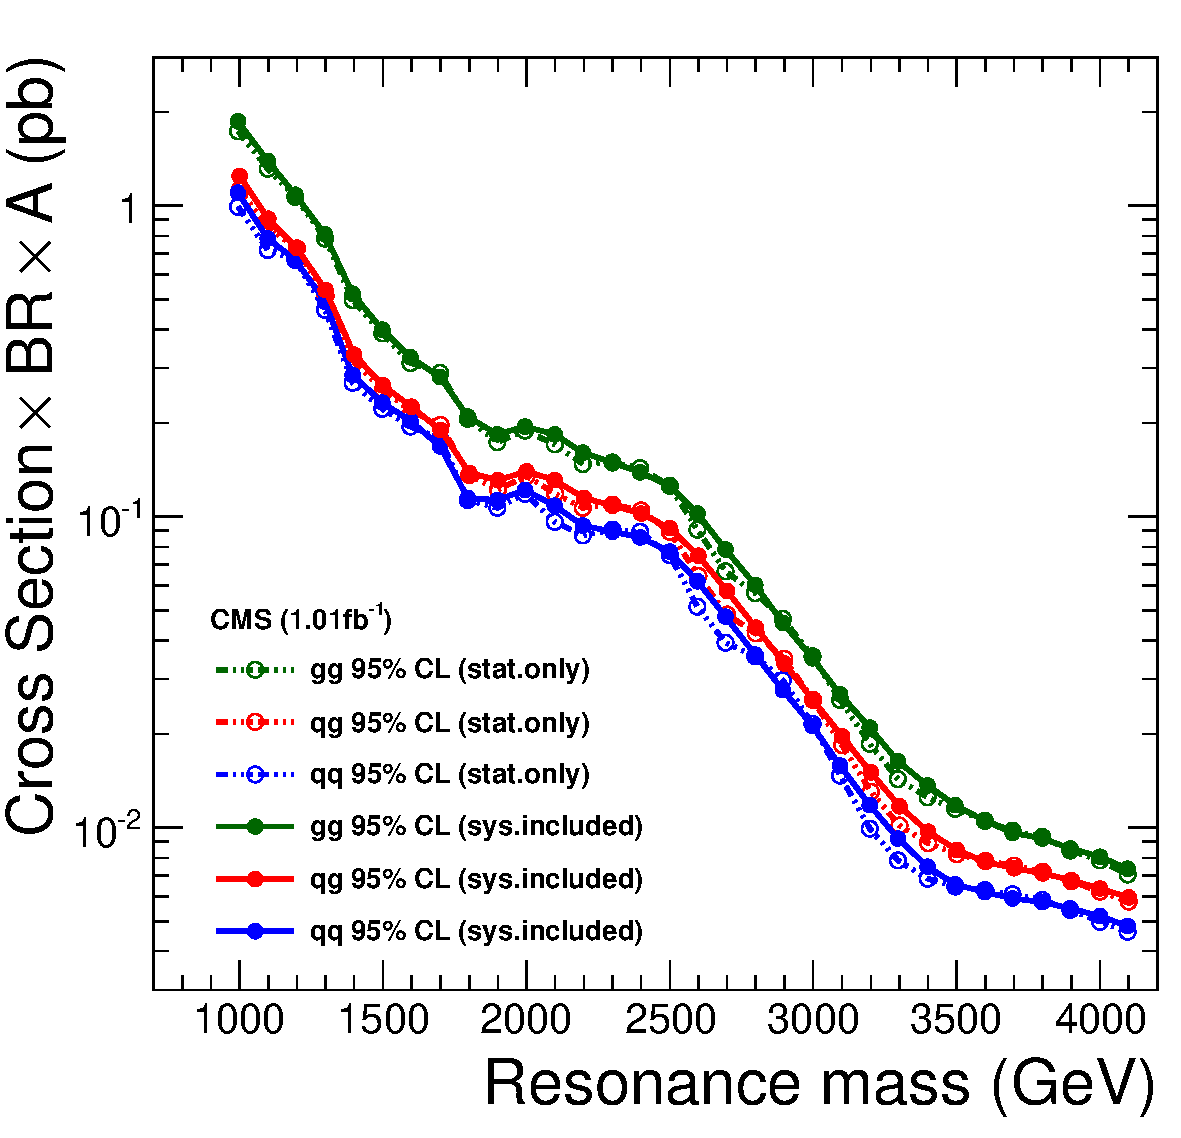
\includegraphics[width=0.48\textwidth]{Figures/c_xs_all_fat.pdf}
    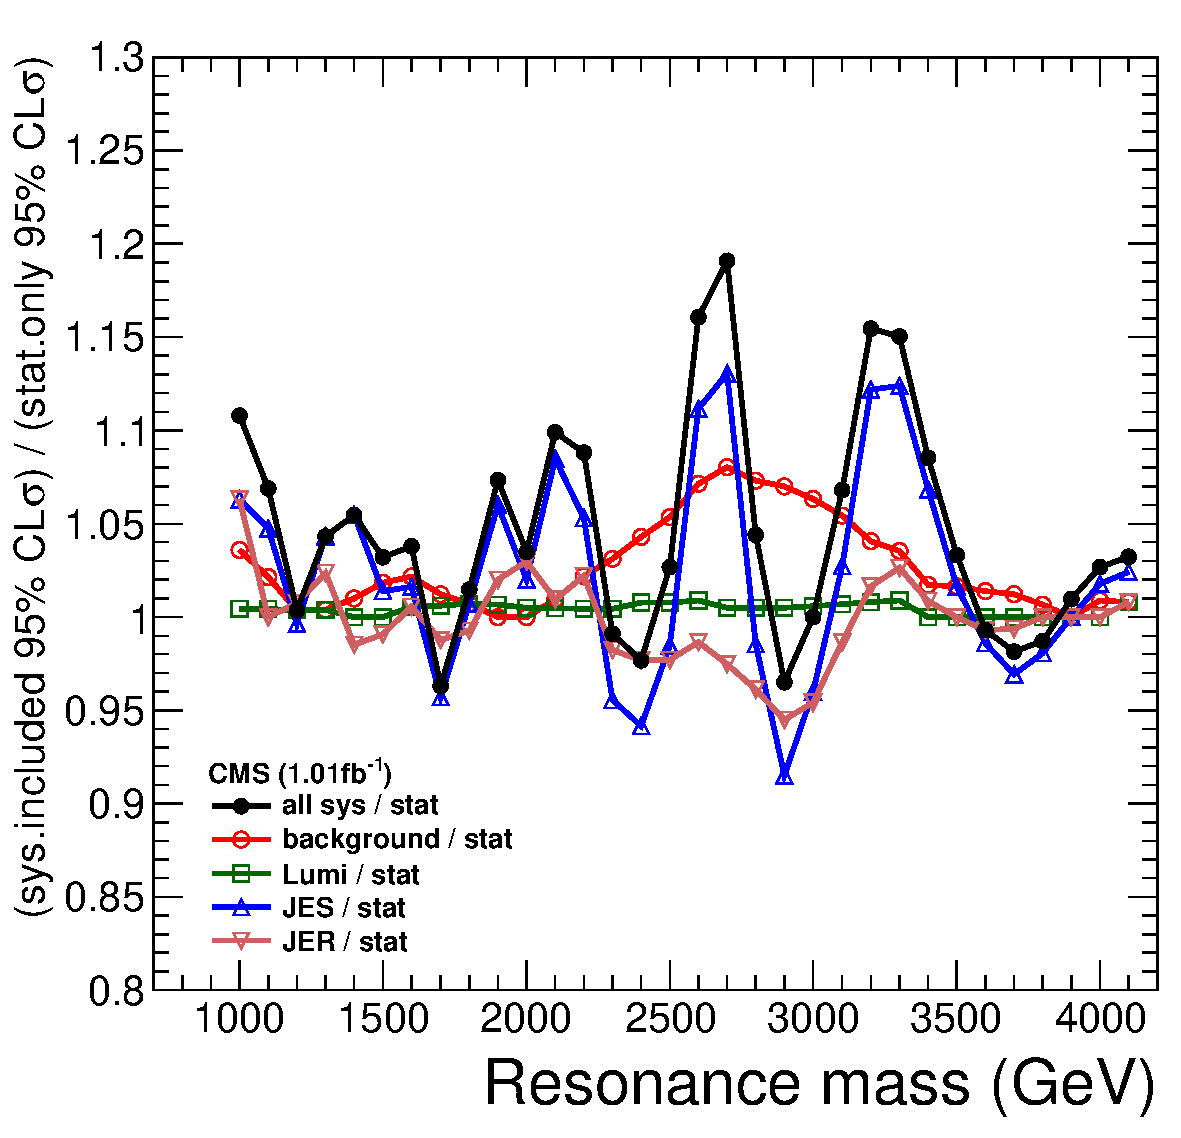
\includegraphics[width=0.48\textwidth]{Figures/c_xs_comparison_bw_stat_sys_fat.pdf}
    \caption{Left) Limits on qg resonances with and without all systematic uncertainties for fat jets. 
    Right) Fractional change in the limit after including systematics.}
    \label{limit_change_fat}
  \end{center}
\end{figure}

\begin{figure}[!ht]
  \begin{center}
     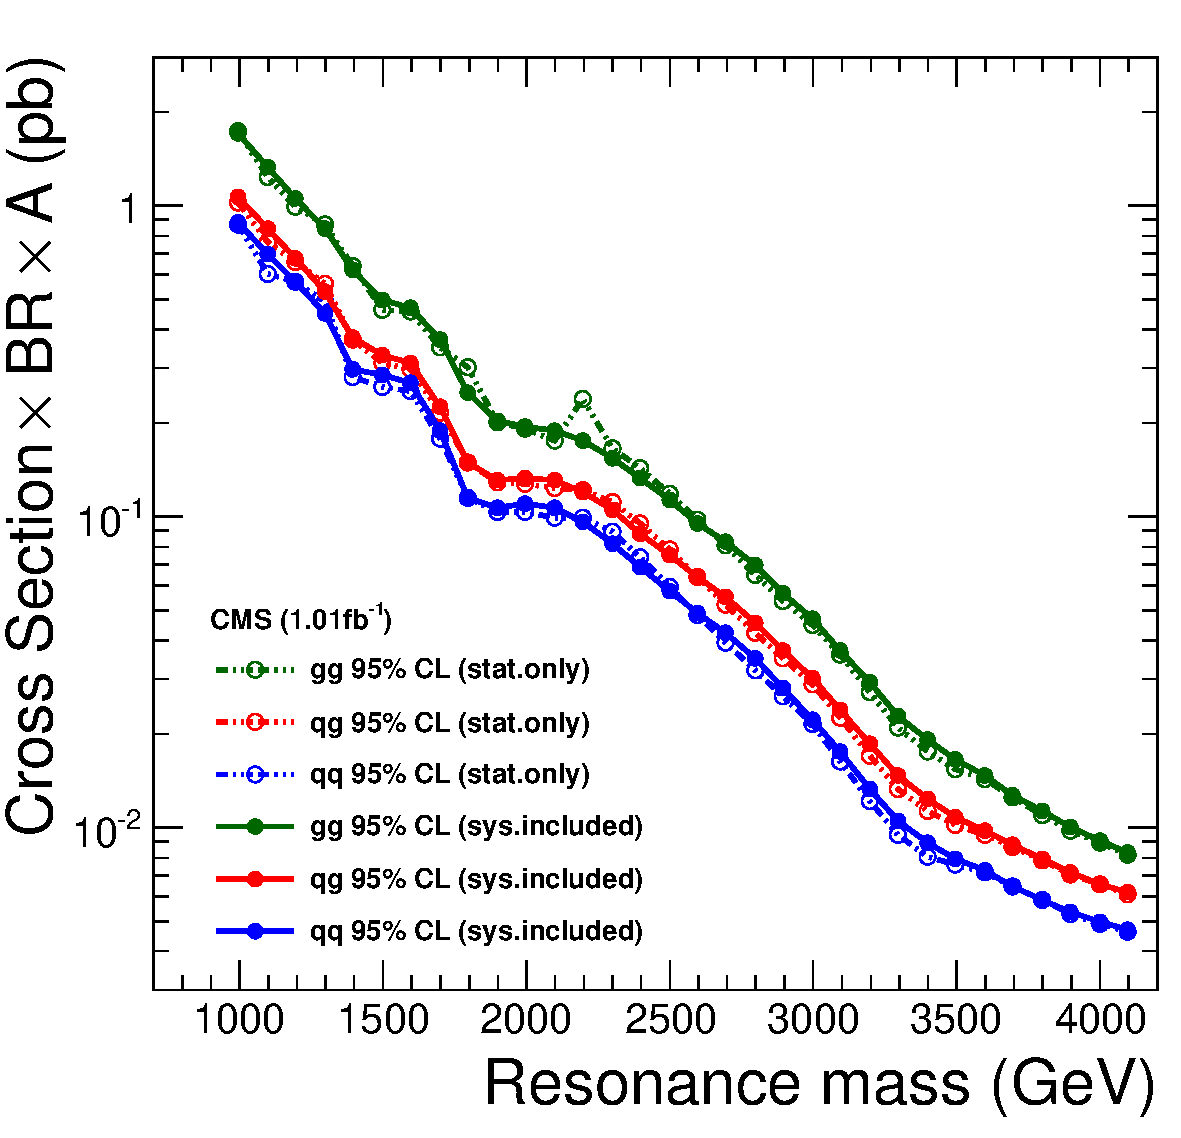
\includegraphics[width=0.48\textwidth]{Figures/c_xs_all_pf.pdf}
    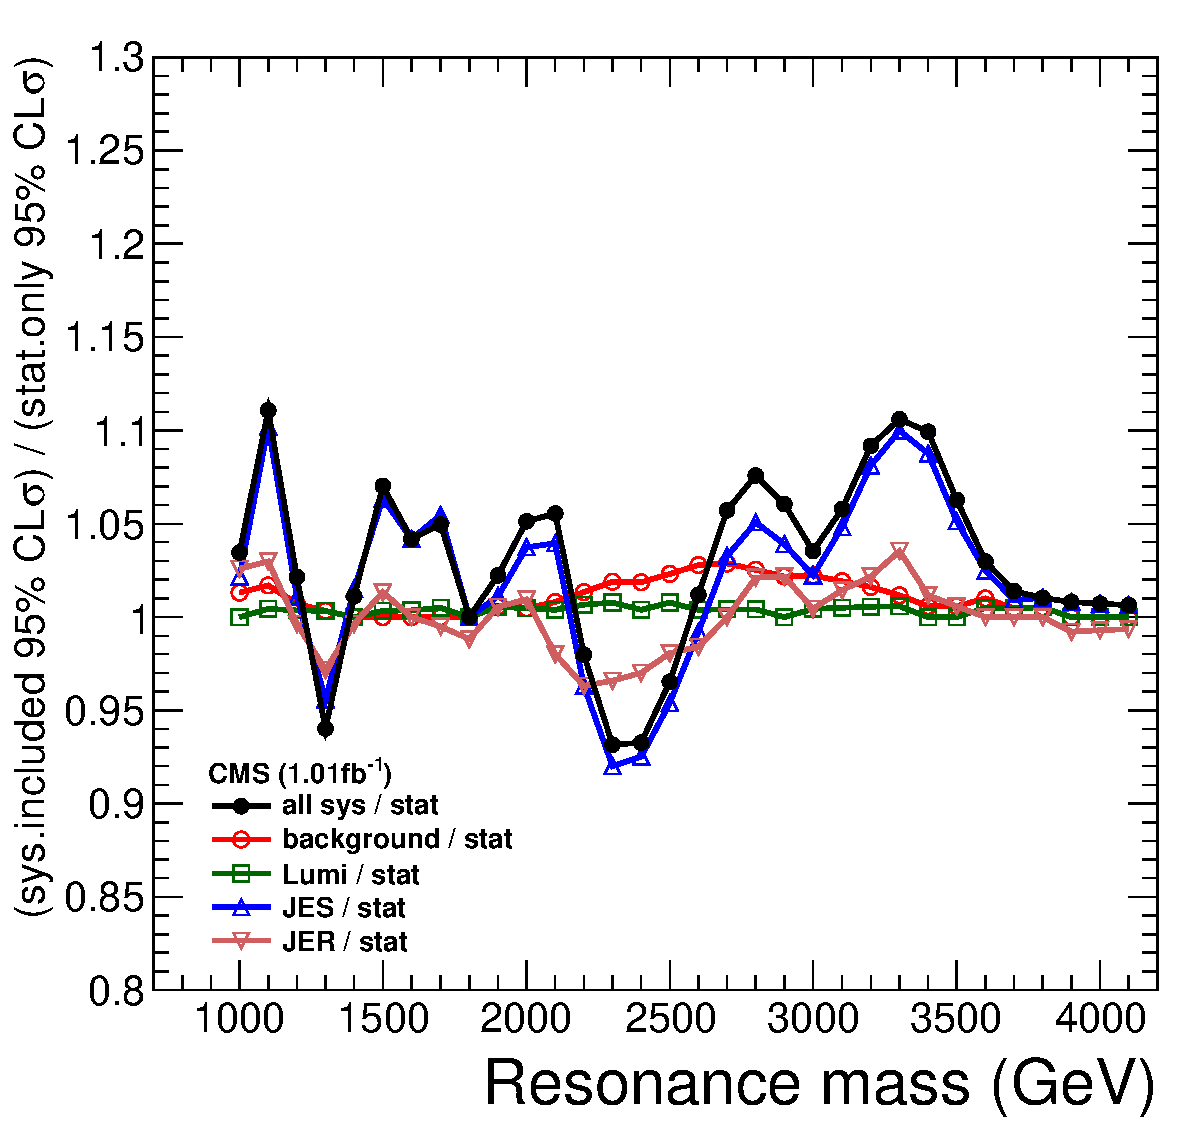
\includegraphics[width=0.48\textwidth]{Figures/c_xs_comparison_bw_stat_sys_pf.pdf}
    \caption{Left) Limits on qg resonances with and without all systematic uncertainties for pf jets. 
    Right) Fractional change in the limit after including systematics.}
    \label{limit_change_pf}
  \end{center}
\end{figure}

\begin{figure}[!ht]
  \begin{center}
     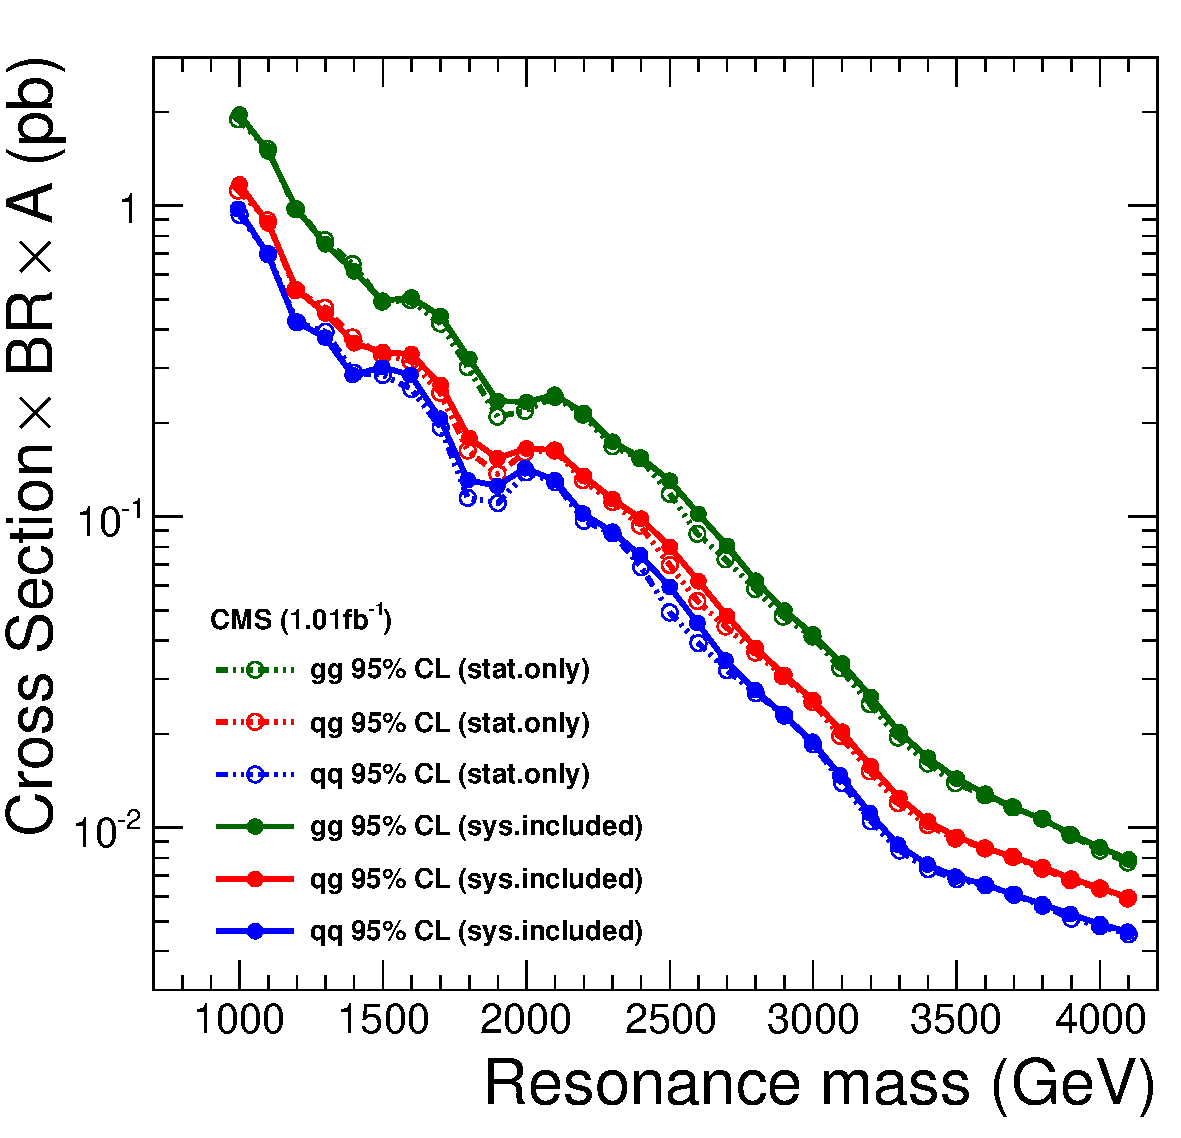
\includegraphics[width=0.48\textwidth]{Figures/c_xs_all_calo.pdf}
    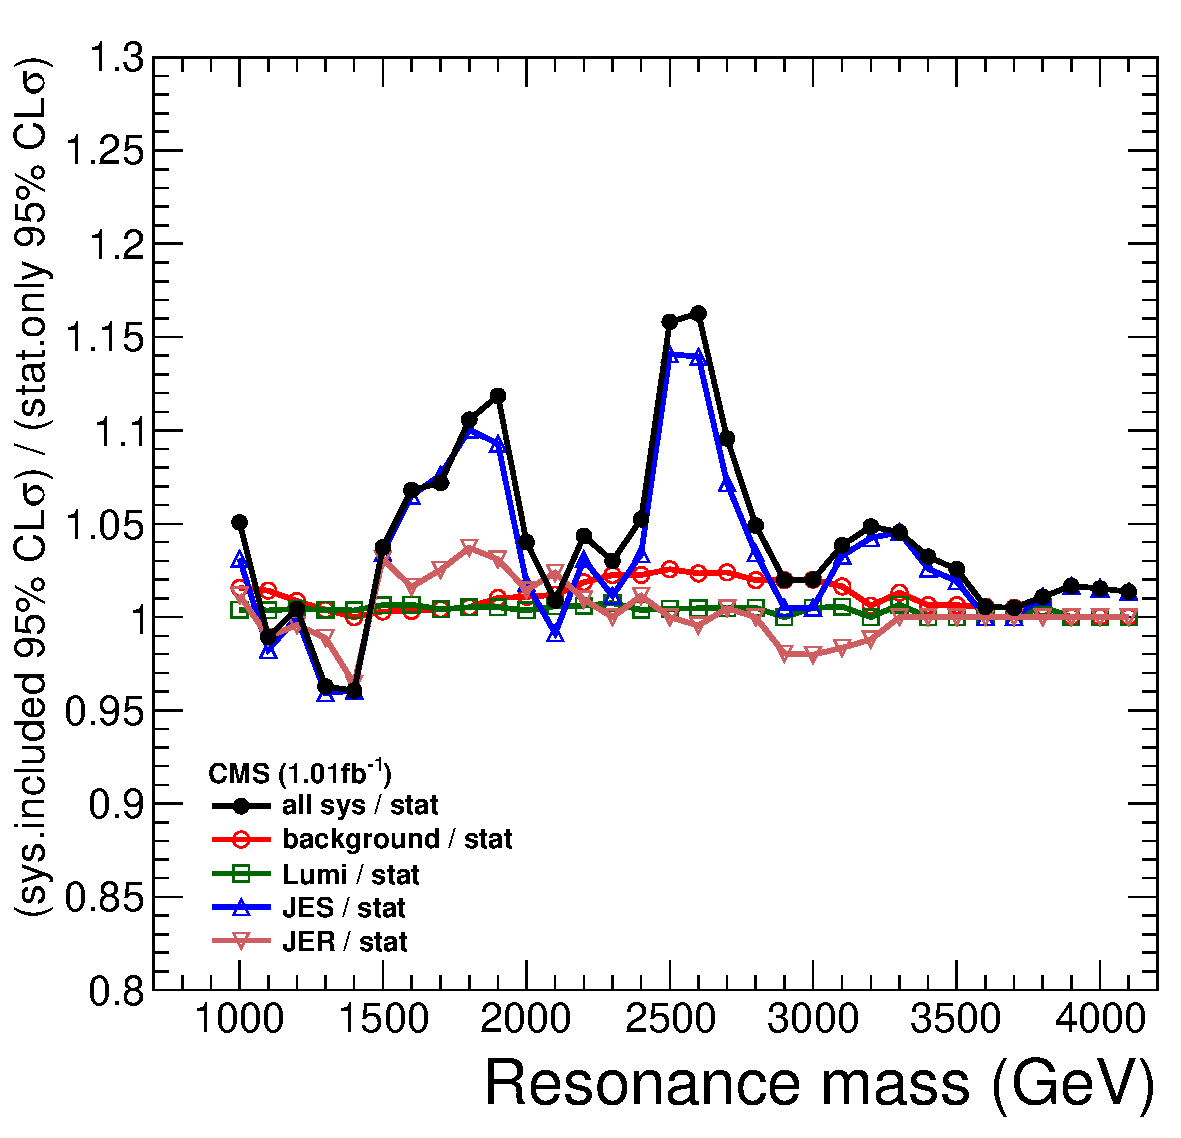
\includegraphics[width=0.48\textwidth]{Figures/c_xs_comparison_bw_stat_sys_calo.pdf}
    \caption{Left) Limits on qg resonances with and without all systematic uncertainties for calo jets. 
    Right) Fractional change in the limit after including systematics.}
    \label{limit_change_calo}
  \end{center}
\end{figure}

\clearpage

\begin{table}[htbH]
\centering
\large
\begin{tabular}{|c|c|c|c|}\hline
Mass   &  \multicolumn{3}{c|}{95\% C.L. $\sigma\cdot B$ (pb) Stat. Err. Only}\\
 ($TeV$) & quark-quark       & quark-gluon  & gluon-gluon\\ \hline
1.0 & 1.09798 & 1.24529 & 1.85078 \\
1.1 & 0.77656 & 0.90878 & 1.37366 \\
1.2 & 0.66212 & 0.73244 & 1.07897 \\
1.3 & 0.48566 & 0.53490 & 0.80296 \\
1.4 & 0.28418 & 0.33180 & 0.51830 \\
1.5 & 0.23093 & 0.26478 & 0.39515 \\
1.6 & 0.20144 & 0.22591 & 0.32564 \\
1.7 & 0.16784 & 0.18973 & 0.28033 \\
1.8 & 0.11464 & 0.13806 & 0.20666 \\
1.9 & 0.11287 & 0.13121 & 0.18334 \\
2.0 & 0.12136 & 0.13984 & 0.19315 \\
2.1 & 0.10792 & 0.13001 & 0.18302 \\
2.2 & 0.09337 & 0.11510 & 0.15953 \\
2.3 & 0.08928 & 0.10847 & 0.14763 \\
2.4 & 0.08536 & 0.10217 & 0.13774 \\
2.5 & 0.07666 & 0.09185 & 0.12474 \\
2.6 & 0.06192 & 0.07487 & 0.10108 \\
2.7 & 0.04696 & 0.05766 & 0.07810 \\
2.8 & 0.03560 & 0.04404 & 0.06010 \\
2.9 & 0.02736 & 0.03363 & 0.04548 \\
3.0 & 0.02097 & 0.02569 & 0.03484 \\
3.1 & 0.01577 & 0.01965 & 0.02678 \\
3.2 & 0.01178 & 0.01507 & 0.02090 \\
3.3 & 0.00908 & 0.01169 & 0.01628 \\
3.4 & 0.00747 & 0.00968 & 0.01364 \\
3.5 & 0.00651 & 0.00847 & 0.01173 \\
3.6 & 0.00612 & 0.00776 & 0.01049 \\
3.7 & 0.00592 & 0.00739 & 0.00957 \\
3.8 & 0.00571 & 0.00712 & 0.00913 \\
3.9 & 0.00547 & 0.00678 & 0.00843 \\
4.0 & 0.00516 & 0.00638 & 0.00799 \\
4.1 & 0.00480 & 0.00597 & 0.00732 \\
\hline
\end{tabular}
\caption{As a function of resonance mass we list our 95\% C.L. upper limit on
cross section times branching ratio for narrow resonances originating from
quark-quark, quark-gluon and gluon-gluon pairs of partons, 
including all systematic errors for wide jets.}
\label{tabSysLimit_calo}
\end{table}

\clearpage


\begin{table}[htbH]
\centering
\large
\begin{tabular}{|c|c|c|c|}\hline
Mass   &  \multicolumn{3}{c|}{95\% C.L. $\sigma\cdot B$ (pb) Stat. Err. Only}\\
 ($TeV$) & quark-quark       & quark-gluon  & gluon-gluon\\ \hline
1.0 & 0.88283 & 1.05836 & 1.68674 \\
1.1 & 0.69751 & 0.83665 & 1.32348 \\
1.2 & 0.56792 & 0.66876 & 1.04411 \\
1.3 & 0.44544 & 0.52613 & 0.84110 \\
1.4 & 0.29422 & 0.37231 & 0.61770 \\
1.5 & 0.28209 & 0.32928 & 0.49145 \\
1.6 & 0.26669 & 0.30755 & 0.46915 \\
1.7 & 0.18677 & 0.22426 & 0.36805 \\
1.8 & 0.11481 & 0.14837 & 0.24845 \\
1.9 & 0.10563 & 0.13092 & 0.20140 \\
2.0 & 0.10940 & 0.13258 & 0.19480 \\
2.1 & 0.10574 & 0.12942 & 0.18710 \\
2.2 & 0.09512 & 0.11896 & 0.17395 \\
2.3 & 0.08195 & 0.10374 & 0.15302 \\
2.4 & 0.06858 & 0.08815 & 0.13120 \\
2.5 & 0.05738 & 0.07473 & 0.11167 \\
2.6 & 0.04898 & 0.06372 & 0.09471 \\
2.7 & 0.04196 & 0.05461 & 0.08223 \\
2.8 & 0.03456 & 0.04542 & 0.06876 \\
2.9 & 0.02771 & 0.03690 & 0.05632 \\
3.0 & 0.02217 & 0.02981 & 0.04625 \\
3.1 & 0.01736 & 0.02361 & 0.03709 \\
3.2 & 0.01314 & 0.01843 & 0.02910 \\
3.3 & 0.01042 & 0.01451 & 0.02270 \\
3.4 & 0.00888 & 0.01228 & 0.01900 \\
3.5 & 0.00794 & 0.01078 & 0.01652 \\
3.6 & 0.00718 & 0.00970 & 0.01464 \\
3.7 & 0.00645 & 0.00869 & 0.01270 \\
3.8 & 0.00581 & 0.00783 & 0.01125 \\
3.9 & 0.00530 & 0.00708 & 0.00992 \\
4.0 & 0.00492 & 0.00656 & 0.00899 \\
4.1 & 0.00463 & 0.00612 & 0.00820 \\
\hline
\end{tabular}
\caption{As a function of resonance mass we list our 95\% C.L. upper limit on
cross section times branching ratio for narrow resonances originating from
quark-quark, quark-gluon and gluon-gluon pairs of partons, 
including all systematic errors for PF jets.}
\label{tabSysLimit_pf}
\end{table}

\clearpage

\begin{table}[htbH]
\centering
\large
\begin{tabular}{|c|c|c|c|}\hline
Mass   &  \multicolumn{3}{c|}{95\% C.L. $\sigma\cdot B$ (pb) Stat. Err. Only}\\
 ($TeV$) & quark-quark       & quark-gluon  & gluon-gluon\\ \hline
1.0 & 0.96805 & 1.17069 & 1.96624 \\
1.1 & 0.69486 & 0.87632 & 1.49566 \\
1.2 & 0.42347 & 0.53599 & 0.97495 \\
1.3 & 0.37404 & 0.45000 & 0.75208 \\
1.4 & 0.28432 & 0.36109 & 0.61430 \\
1.5 & 0.30171 & 0.33838 & 0.49420 \\
1.6 & 0.28368 & 0.33327 & 0.50799 \\
1.7 & 0.20581 & 0.26488 & 0.44072 \\
1.8 & 0.13015 & 0.17869 & 0.32184 \\
1.9 & 0.12509 & 0.15220 & 0.23335 \\
2.0 & 0.14135 & 0.16546 & 0.23366 \\
2.1 & 0.12970 & 0.16371 & 0.24583 \\
2.2 & 0.10190 & 0.13509 & 0.21530 \\
2.3 & 0.08848 & 0.11422 & 0.17454 \\
2.4 & 0.07481 & 0.09837 & 0.15441 \\
2.5 & 0.05885 & 0.07986 & 0.13043 \\
2.6 & 0.04506 & 0.06189 & 0.10175 \\
2.7 & 0.03430 & 0.04789 & 0.08052 \\
2.8 & 0.02760 & 0.03785 & 0.06227 \\
2.9 & 0.02306 & 0.03100 & 0.05002 \\
3.0 & 0.01878 & 0.02576 & 0.04187 \\
3.1 & 0.01452 & 0.02032 & 0.03366 \\
3.2 & 0.01103 & 0.01577 & 0.02635 \\
3.3 & 0.00873 & 0.01244 & 0.02025 \\
3.4 & 0.00760 & 0.01048 & 0.01677 \\
3.5 & 0.00693 & 0.00932 & 0.01439 \\
3.6 & 0.00653 & 0.00859 & 0.01287 \\
3.7 & 0.00608 & 0.00802 & 0.01160 \\
3.8 & 0.00564 & 0.00745 & 0.01063 \\
3.9 & 0.00521 & 0.00685 & 0.00951 \\
4.0 & 0.00486 & 0.00639 & 0.00863 \\
4.1 & 0.00457 & 0.00597 & 0.00790 \\
\hline
\end{tabular}
\caption{As a function of resonance mass we list our 95\% C.L. upper limit on
cross section times branching ratio for narrow resonances originating from
quark-quark, quark-gluon and gluon-gluon pairs of partons, 
including all systematic errors for calo jets.}
\label{tabSysLimit_fat}
\end{table}

\clearpage
